\section{Introduction}
\label{sec:intro}



{\color{red} TODO: Some Security Background}



VirusTotal provides a valuable resource to study and 
understand real-world malwares and anti-virus engines. 

First, there are huge amount of suspicious files submitted to VirusTotal. 
As shown in Figure~\ref{fig:subnum}, 
there are around 40 million submissions on VirusTotal each month. 
These submissions cover a large variety of file types, and 
are conducted by a large variety of VirusTotal users from all over the world. 
This amount of diverse data on VirusTotal serves as a good representation of malwares in the real world.  

Second, for around all submissions, 
VirusTotal applies no less than 50 state-of-the-art anti-virus engines to analyze them. 
VirusTotal keeps detailed detection results, and provide access to these results. 
Analyzing historical detection results can help capture how anti-virus engines evolve over time. 

Third, VirusTotal provides rich metadata for each submission. 
Besides detection results from different engines, 
VirusTotal also provides file type information, which can help categorize malwares, 
source ID (country), which can help understand popularity of malwares, 
ssdeep digest string, by using which we can calculate code similarity without accessing binary executable, and so on. 


{\color{red} TODO: Existing works on VirusTotal}



\begin{figure}[t!]
\begin{center}
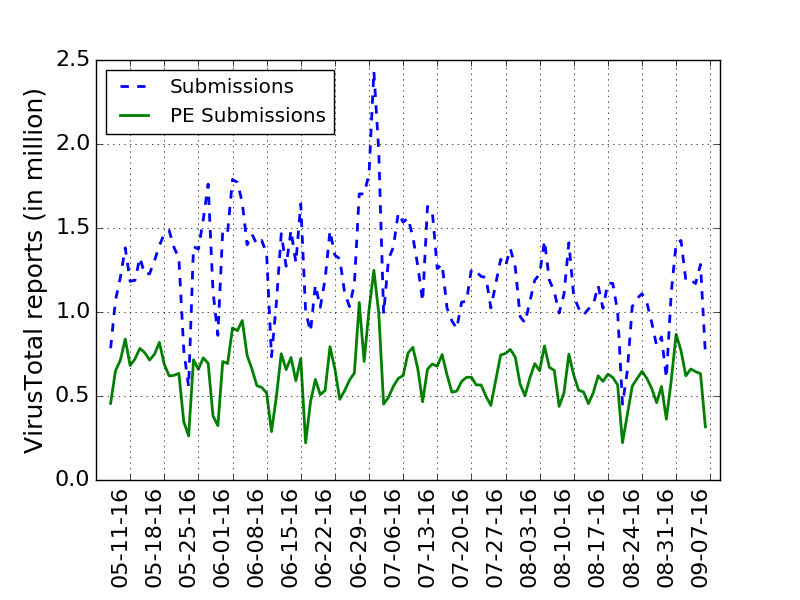
\includegraphics[width=2in]{figure/Submissions}
\caption{The number of files and PE files.
%{\footnotesize{
(The number of suspicious files and the number of PE files submitted to VirusTotal from 05/07/2016 to 09/06/2016.)
%}
}
\label{fig:subnum}
\end{center}
%\vspace{-0.25in}
\end{figure}


In this paper, we collect 4-month metadata from VirusTotal,
and conduct a thorough study on these data. 
Following previous works~\cite{SongAPsys2016} on studying VirusTotal,
we focus our effort on PE files, 
which occupy more than half of VirusTotal’s submissions.
Our study can improve the understanding of malwares and anti-virus engines in the real world, 
and provide implications for future works to 
apply machine learning to malware detection in a large scale. 
Our study is mainly conducted in three aspects: 


First, we study the correlation between submissions’ metadata and their detection rates. 
Given a submission, 
we calculate its detection rate as the percentage of engines 
labeling the submission as malware. 
Higher detection rate indicates a more malicious submission viewed by engines.  
We study correlation between detection rate 
and source ids’ reputation, submission history, file size and source country. 
Our studying results can help categorize which types of malwares are more malicious, 
help security experts invest their limited manual efforts, 
and help anti-virus vendors identify possible false positives and false negatives in their products.   


Second, we study how influence propagate among different anti-virus vendors. 
Anti-virus vendors frequently leverage VirusTotal to identify false negatives in their products, 
which are malwares detected by others’ products, 
but not detected by their own products. 
We assume there is influence among each pair of vendors. 
By using detection history from VirusTotal, 
we train 4 static models from web mining area to quantize this influence. 
Our trained models can be used to evaluate which vendors are more influential in security community. 
We also use our trained models to predict whether a vendor will label a submitted file as malware, 
after it previously labeled the file as benign. 
Anti-virus vendors can rely on this technique to identify false negatives in their products. 

Third, we explore the feasibility to build malware classifiers or detectors based on ssdeep similarity. 
For each submission, ssdeep hash string is also provided by VirusTotal. 
The similarity between two ssdeep hash strings 
is a good estimation of similarity between the two original binary files.
Hash strings can be automatically calculated by ssdeep programs. 
If we can build malware detectors by using ssdeep hash strings, 
we can avoid manually extract signatures from malware samples.   
We design several experiments to evaluate our ssdeep-based malware classifiers. 
Our evaluation results show that precision of malware classifiers are 
bounded by percentage of tailing examples and more training data tends to bring better results.

{\color{red} TODO: Contributions:}